\Chapter{Lekérdezések optimalizálása}

Az alap ötlet egyszerű. A \texttt{MySQL} szerverről lekérjük a tábla tartalmát, amit bemásolunk az \textit{OpenCL} pufferébe, majd a kernelkód futtatása után az eredményt tartalmazó részeket kiolvassuk. Felvetődik azonban néhány problémás rész.
\begin{itemize}
	\item Hogyan tároljuk a tábla tartalmát?
	\item Mekkora legyen a Globális munkaméret és a munkacsoport méret?
	\item Milyen formában állítsuk elő az eredményt, és hogyan olvassuk azt ki?
\end{itemize}
A fejezetben ezen kérdések vizsgálatára és megválaszolására kerül sor.

\Section{Adatok előkészítése}

Az adatok feldolgozása egy többlépéses folyamat. A lekérdezés végrehajtása előtt előkészítő lépésekre van szükség.

\SubSection{Táblák tömbbé alakítása}

Ahhoz, hogy \textit{OpenCL} -el kezelni tudjuk az adatokat először szükségünk lesz egy struktúrára, ami reprezentálja az adatbázis tábla felépítését, azaz a struktúra adattagjainak típusa egyezzen meg a táblázat oszlopainak típusával. Ezek után ebből létre kell hoznunk egy tömböt, melynek hossza legalább annyi, mint a tábla sorainak száma (\ref{fig:structure}. ábra).

\begin{figure}[h!]
\centering
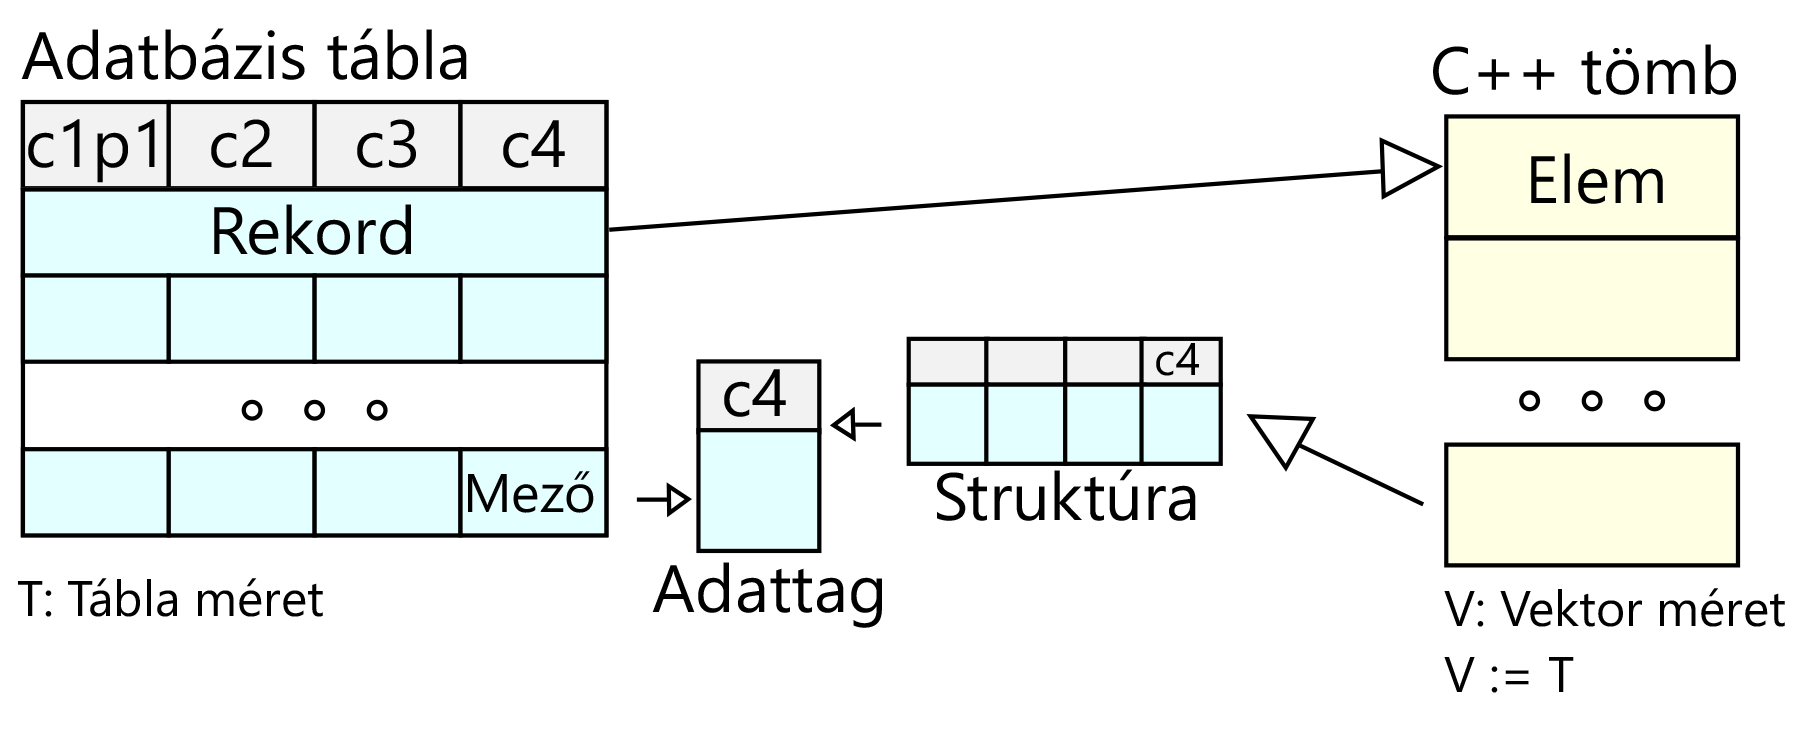
\includegraphics[width=11cm]{images/data/structure.png}
\caption{Adatbázistábla átalakítása tömbbé}
\label{fig:structure}
\end{figure}

A következőket érdemes figyelembe venni:
\begin{itemize}
\item A struktúra megfelel a tábla felépítésének.
\item A tömb típusa egy ilyen struktúra.
\item A tömb egy eleme megfelel a tábla egy rekordjának azaz sorának.
\item Egy elem adattagjai megfelelnek az adatbázis egyazon rekordjához tartozó mezőknek.
\end{itemize}

\SubSection{A táblákat beolvasó függvény.}

A fix sorszámmal rendelkező adatbázis táblák kezelése egy nagyon speciális eset lenne, ezért a programot úgy kell megírni, hogy igazodni tudjon a különböző táblaméretekhez.

Mivel a tábla méret előre nem ismert, ezért a tömböket a \texttt{malloc} függvénnyel lehet lefoglalni. Mivel a lekérdezést külön függvény végzi, és a méretet sem tudjuk előre, ezért a következő megoldást alkalmazom.

Első lépésben létrehozok egy pointert, ami később a táblára fog mutatni, most még \texttt{NULL} értékű, és ehhez egy változót ami a méretet tárolja. Az adatokat lekérő függvénynek átadom ezeket, és miután a \texttt{Connector} elvégezte a lekérdezést beállítom a méret változó értékét, illetve a tábla memória területét csak ekkor foglalom le, és állítom rá a pointert. Ez úgy lehetséges, hogy a függvénynek egy pointerre mutató pointert adok át, ezáltal kettős indirektség jön létre (\ref{fig:pointer_01}. és \ref{fig:pointer_02}. ábra).

\begin{cpp}
Table1Type *t1 = NULL;
int t1_size;
load_database(&t1, &t1_size);
res = pstmt->executeQuery();
\end{cpp}
\begin{figure}[h!]
\centering
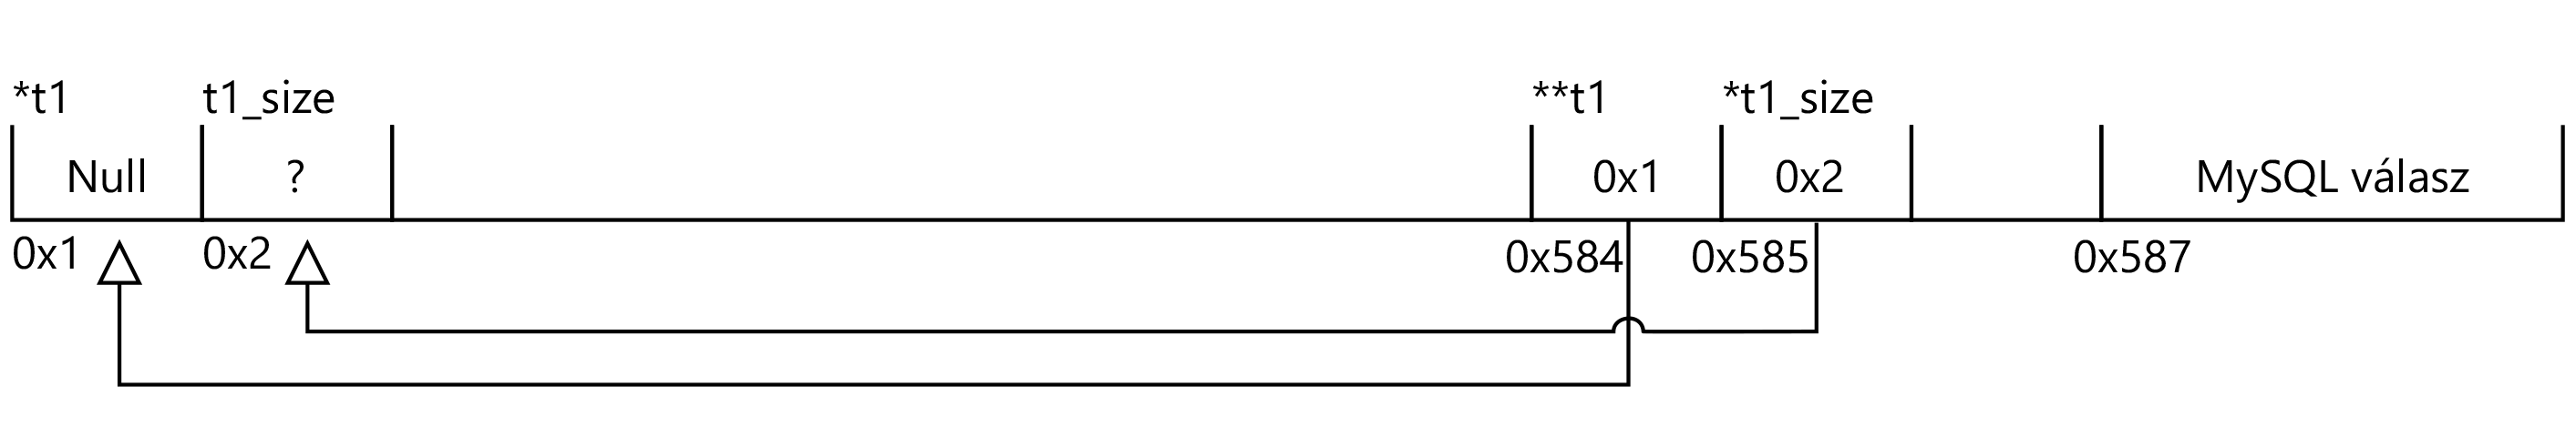
\includegraphics[width=\textwidth]{images/implementation/pointer_01.png}
\caption{Pointerek a létrehozáskor}
\label{fig:pointer_01}
\end{figure}
\begin{cpp}
int i = 0;
*T1_size = res->rowsCount();
*T1 = (Table1Type*) malloc(sizeof(Table1Type) * *T1_size);

while (res->next()) {
    T1[0][i].c1p1 = res->getInt("c1p1");
    T1[0][i].c2 = res->getInt("c2");
    T1[0][i].c3 = res->getInt("c3");
    T1[0][i].c4 = res->getInt("c4");
    i++;
}
\end{cpp}

\begin{figure}[h!]
\centering
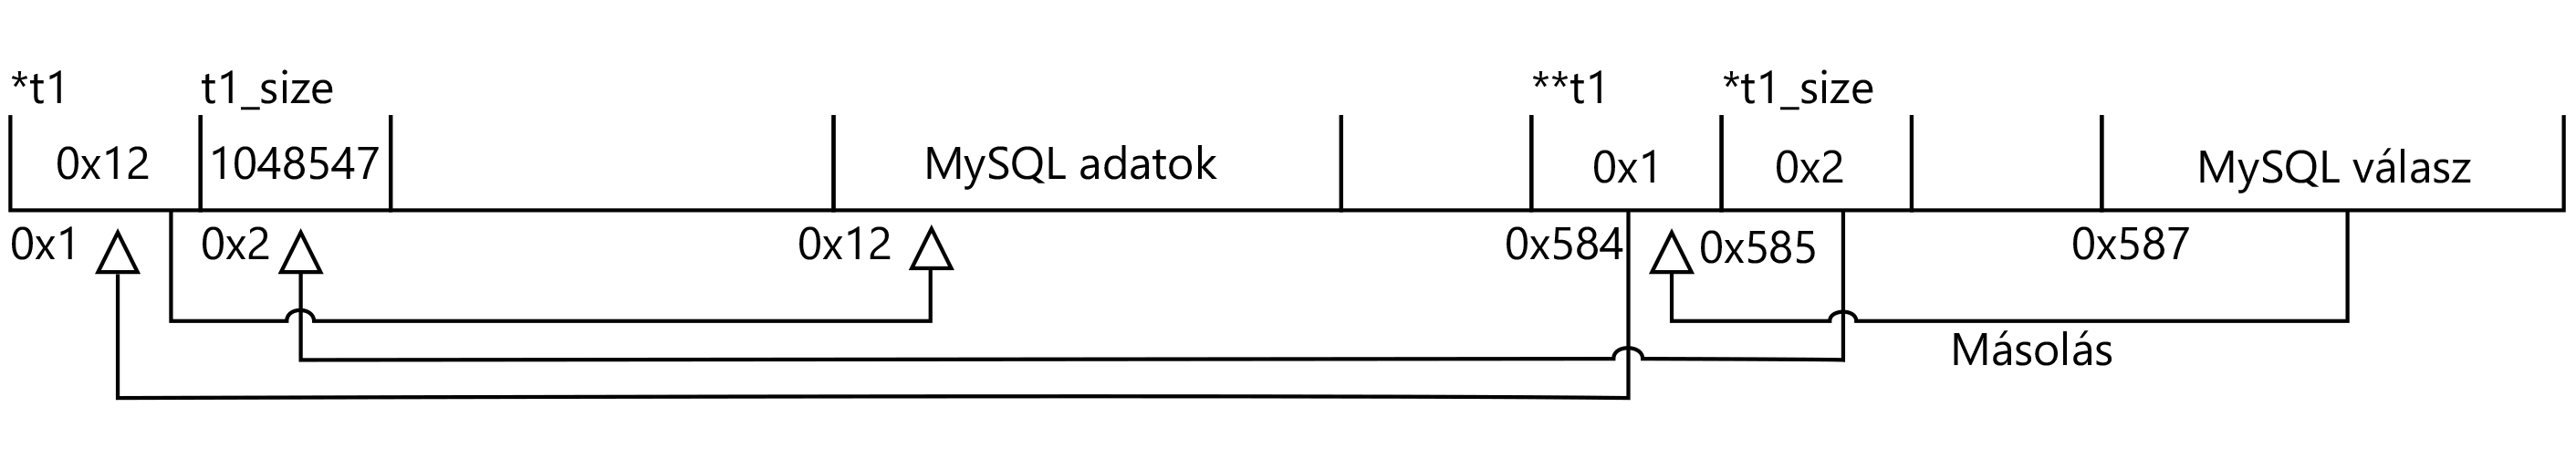
\includegraphics[width=\textwidth]{images/implementation/pointer_02.png}
\caption{Pointerek teljes működése}
\label{fig:pointer_02}
\end{figure}

\noindent (Ennek az implementációját a mellékelt \texttt{cp\_to\_array} nevű programban találjuk.)

\Section{Globális és lokális méret meghatározása}
Ennél a pontnál oda kell figyelni pár alapvető dologra.
\begin{itemize}
\item A lokális méret legfeljebb 1024 lehet.
\item A globális méretnek a lokális többszörösének kell lennie.
\item A túl sok vagy túl kevés munkacsoport használata esetén a párhuzamosság sérül.
\item A munkacsoportok és csoporton belül a munkaelemek feldolgozása párhuzamos.
\item Munkacsoportok között nem lehetséges szinkronizáció, csak munka elemek között, amennyiben azok egy munkacsoportba tartoznak.
\item Nem használható kölcsönös kizárás, a szemafor végtelen ciklushoz vezet.
\end{itemize}

\SubSection{Működési elv}

Egyszerű esetben a bementi elemszámot megadhatjuk, mint globális méret, ez a gyakorlatban meghatározza, hogy hányszor fog lefutni a kernel függvény.

A \texttt{get\_global\_id(0)} meghívásával megkapjuk az aktuális azonosítót, ez 0-tól (globális méret-1)-ig terjed. Innentől tekinthetünk a teljes kódra úgy, mintha egy párhuzamos futó \texttt{for} ciklusban lenne.

Ezen kívül meg kell adnunk a lokális méretet, ami az elemek száma egy munkacsoporton belül. A kernel futása közben ezt is megkaphatjuk a \texttt{get\_local\_id(0)} használatával, csak úgy, mint a munkacsoport azonosítót vagy az említett paraméterek méretét (\ref{fig:workgroups_black}. ábra).

A végeredményt tartalmazó kimeneti tömb hossza egyezik a globális mérettel, így nem ütközhetünk bele abba a hibába, hogy két számítási elem ugyanoda próbáljon írni. Amennyiben például az 545. elem megfelel, akkor az indexe és egyéb hozzá tartozó értékek az 545. helyen lesznek a kimeneti tömbben.

\begin{figure}[h!]
\centering
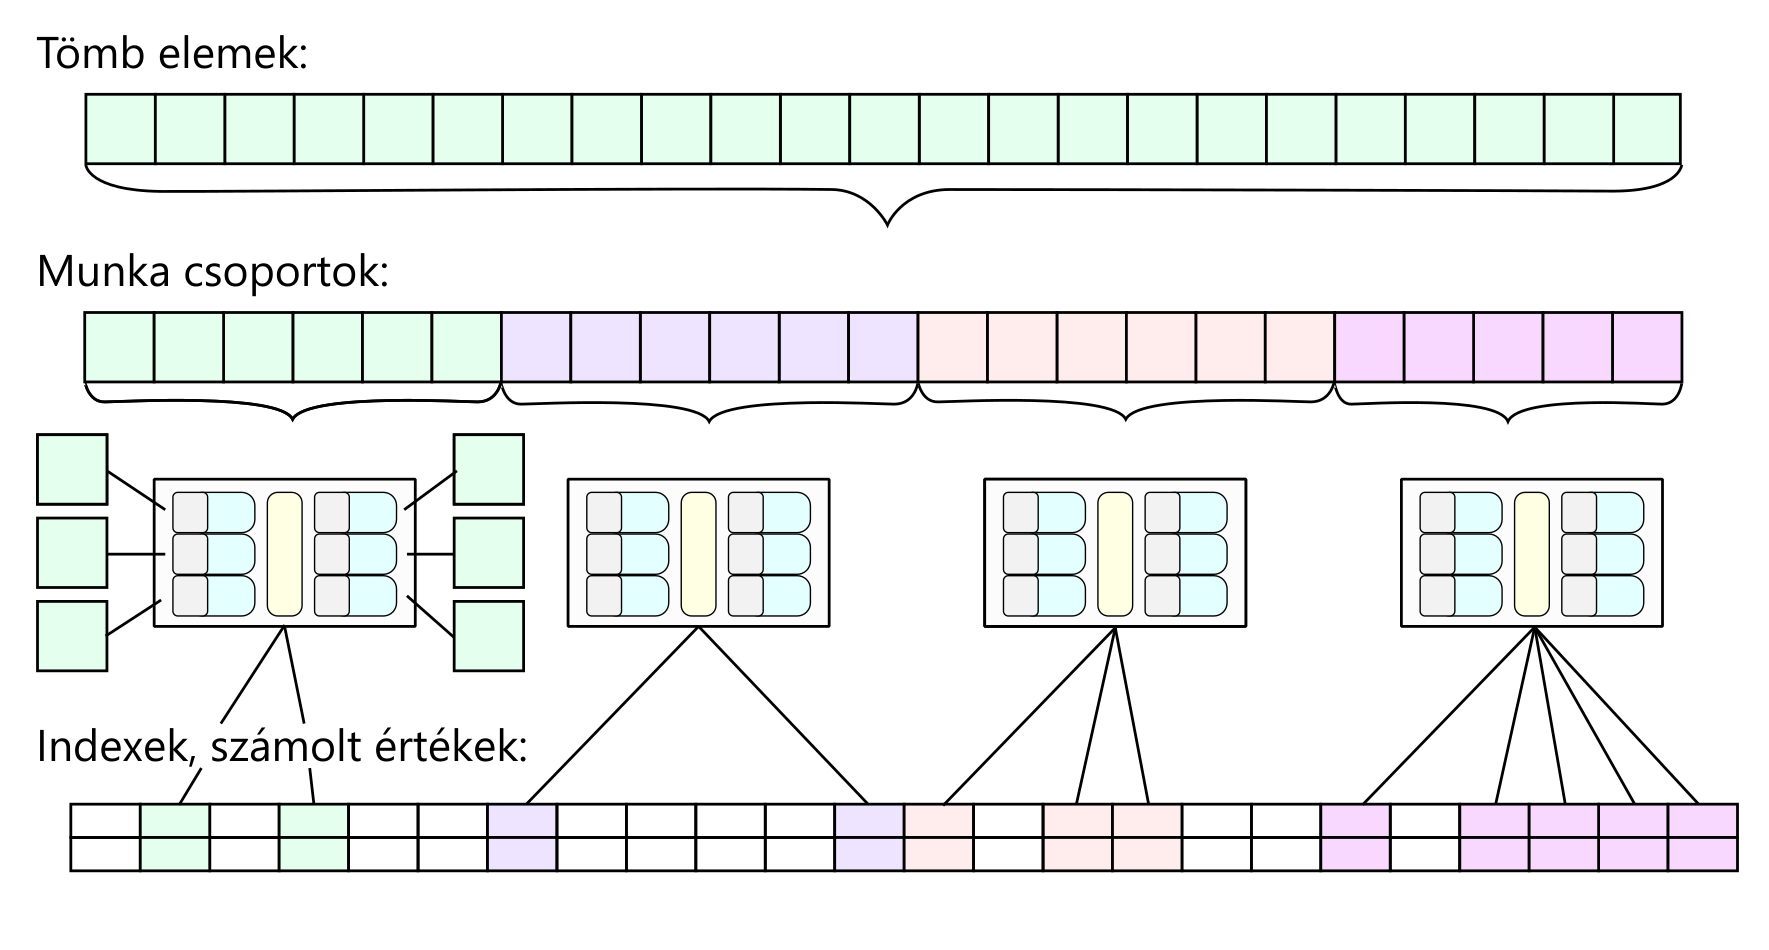
\includegraphics[width=\textwidth]{images/workgroups_black.png}
\caption{Munkacsoportokra bontás}
\label{fig:workgroups_black}
\end{figure}

\newpage

\SubSection{Globális méret meghatározása}

Tegyünk fel, hogy kaptunk egy 1048547 sorból álló táblázatot. Ekkor több probléma is előkerül. Egyrészt olyan lokális méretet kell választani ami ennek a számnak az osztója. Másfelől nem szeretnénk végignézni az ugyan ilyen hosszú kimeneti tömböt az eredmények helyét keresve.

A következő módon oldottam meg a problémát. Állítsuk a globális méretet például 1024-re, ehhez határozzunk meg egy intervallum méretet a sorok száma és globális méret hányadosának felső egész részeként. Ez jelen esetben szintén 1024 lesz. Viszont így át kell adnunk a kernelnek a tábla méretét, ami felső határként ügyel arra, hogy ne lépjük túl a tömböt méretét. A számítás tehát a következő:
\begin{align*}
\text{global\_size} &= 1024, \\
\text{interval\_size} &=
\left\lceil \frac{\text{table\_size}}{\text{globalsize\_size}} \right\rceil.
\end{align*}

A módosításnak az lesz a következménye, hogy egy munkaelem nemcsak a tömb egy elemén fog dolgozni, hanem egy intervallumán. Ezzel létrehoztunk olyan részeket a tömbben, amiknek a feldolgozása biztosan soros lesz. Ennek köszönhetően már tudunk használni számlálókat, nincs szükség kölcsönös kizárásra. A számlálókat tartalmazó tömb mérete megegyezik a globális mérettel.

Ezekhez a paraméterekhez még tetszőlegesen meg kell határozni a lokális méretet, aminek csak a teljesítményre van hatása.

\SubSection{A kernelkód működése}

A kernel meghatározza saját globális azonosítóját és ebből illetve a kapott intervallum méretből kiszámítja, honnan kezdődik az ő része a be-, és kimeneti tömbön. Ezután elkezdi az intervallumnyi elem vizsgálatát ügyelve arra, hogy a tábla méretet ne lépje túl. Amennyiben egy elem megfelel a szűrési paramétereknek annak indexét és egyéb lekérdezés függő kiszámolt értékeket a kimeneti tömbbe másolja, majd növeli saját számlálóját. Ez a számláló határozza meg, hogy a kimeneti szakaszon a következő elem hányadik helyre kerüljön.

\begin{figure}[h!]
\centering
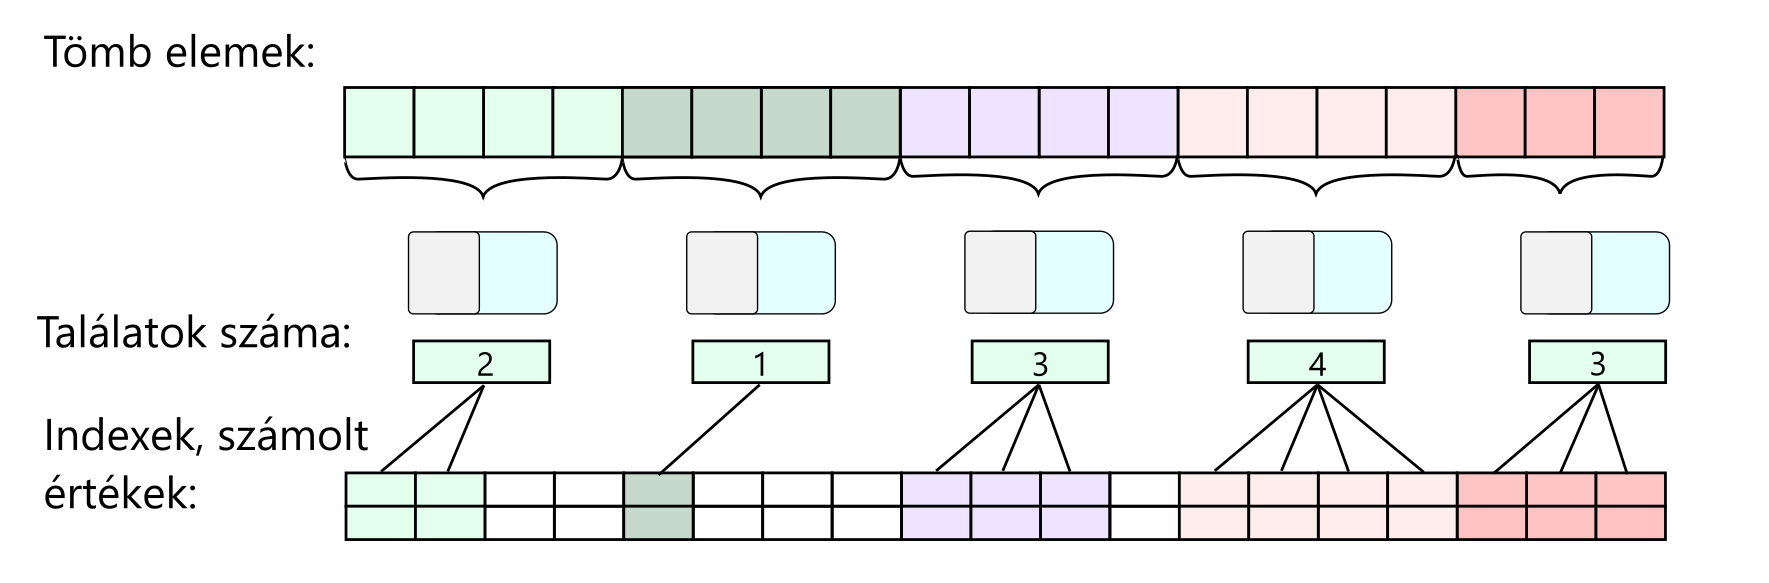
\includegraphics[width=\textwidth]{images/itemgroup_black.png}
\caption{Intervallumok feldolgozása}
\label{fig:itemgroup_black}
\end{figure}

Itt már nem munkacsoportonként, hanem feldolgozó elemenként látjuk a folyamatot (\ref{fig:itemgroup_black}. ábra).

\Section{Eredmény kiolvasása}

A kernelkód működéséből látjuk, hogy több módszert is tudunk alkalmazni az elemek kiolvasására. A találatok számát tartalmazó tömböt biztosan ki kell másolnunk, de kimenetre vonatkozóan nézzük meg az alábbi lehetőségeket. (Az ehhez tartozó kódokat a \texttt{cp\_buffer} nevű programban érdemes megnézni.)

\SubSection{Az elemek kiolvasása egyben}

Dönthetünk úgy, hogy kimásoljuk a teljes kimenetet:
\begin{python}
clStatus = clEnqueueReadBuffer(command_queue, TableResult_clmem, 
    CL_TRUE, 0, table_size * sizeof(TableResultType), result, 
    0, NULL, NULL);
\end{python}
Ekkor ennek olvasása a következőképpen zajlik:
\begin{python}
for (i = 0; i < global_size; i++)
{
    offset = i * interval_size;
    for (j = 0; j < result_counter[i]; j++)
        cout << t1[ result[ offset + j ].index ].c1p1 << endl;
}
\end{python}
Végig kell menni a számlálón, aminek hossza \texttt{global\_size}, majd annyi elemet kell sorban kiolvasni az adott részről \texttt{ i * interval\_size} eltolást használva, amekkora érték a hozzá tartozó számlálóban található. Ezzel végig lépkedve és ugrálva a kimeneten ki tudjuk olvasni az indexeket, illetve kiszámított értékeket.

\SubSection{Az elemek kiolvasása szakaszosan}

A másik módszer, hogy csak az információkat tartalmazó részeket olvassuk a pufferekből. Ez hasonló módon zajlik, mint előző esetben az eredmények kiírása.
\begin{python}
int count = 0;
for (int i = 0; i < global_size; i++)
{
    if (result_counter[i] < 1 ) continue; 
    clStatus = clEnqueueReadBuffer(
    command_queue, TableResult_clmem, CL_TRUE, 
	i * interval_size * sizeof(TableResultType),
	result_counter[i] * sizeof(TableResultType), 
	&result[count], 0, NULL, NULL);
	count += result_counter[i];
}
\end{python}

Kiolvasásnál megadjuk az eltolást, amit az előző módon számolunk annyi különbséggel, hogy megszorozzuk egy elem memória méretével:
\begin{python}
i * interval_size * sizeof(TableResultType)
\end{python}
Ezután megadjuk, hogy az eltolástól kezdve mekkora memória méretet szeretnénk kiolvasni, ezt a számlálóból tudjuk: 
\begin{python}
result_counter[i] * sizeof(TableResultType)
\end{python}
Ezen kívül a másolás cél memóriacímét mindig eltoljuk, az eddigi találatok számával:
\begin{python}
&result[count]
\end{python}
Ha memóriát is szeretnénk spórolni, megtehetjük azt is, hogy először összeadjuk a találatokat és az alapján foglaljuk le a memóriaterületet a kiolvasáshoz (\ref{fig:copy_02}. ábra).

\begin{figure}[h!]
\centering
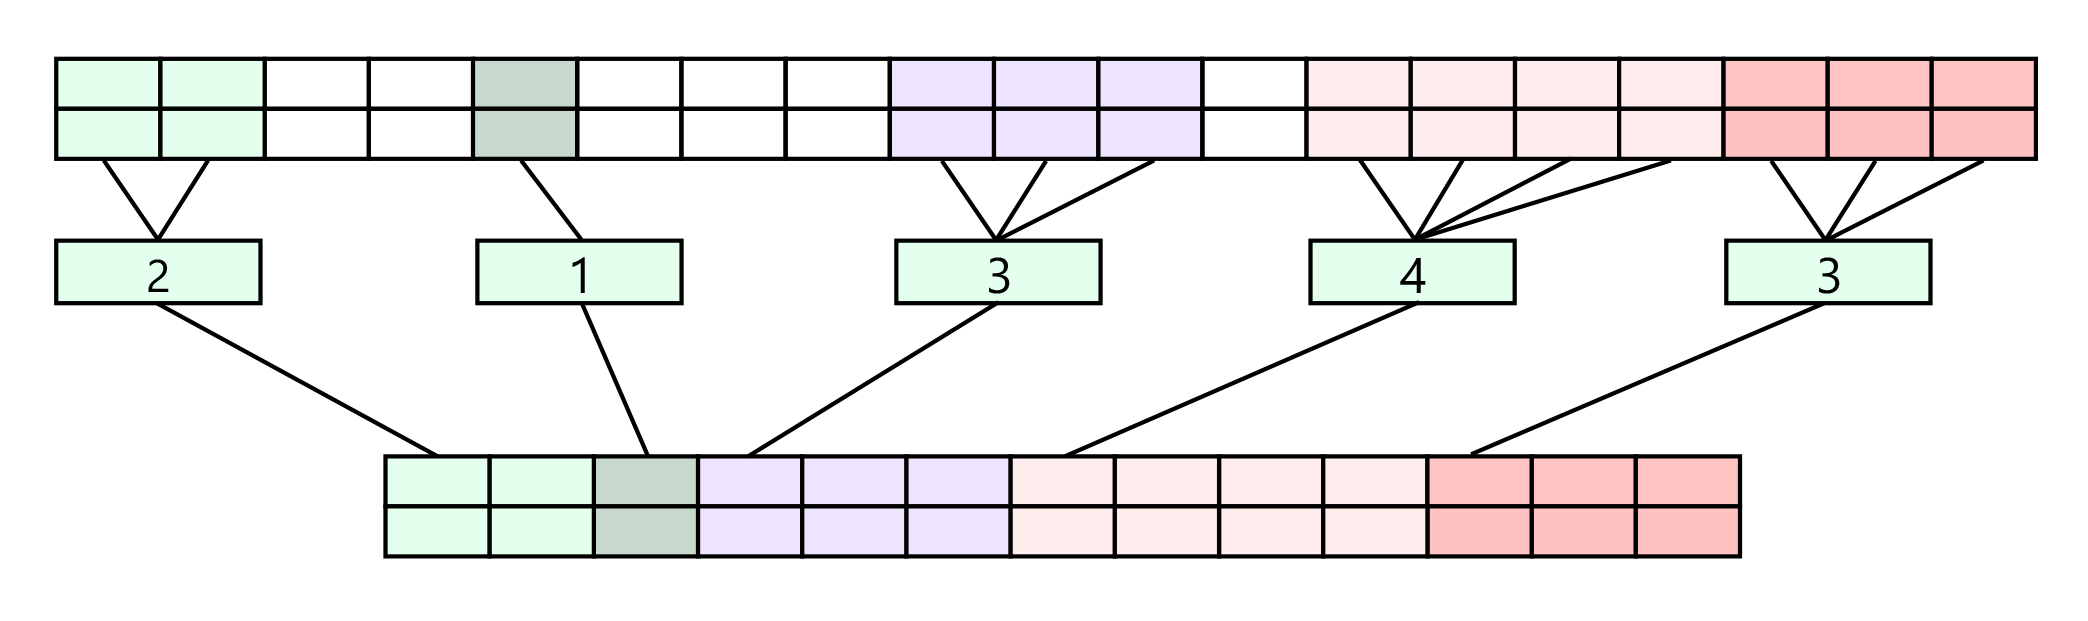
\includegraphics[width=\textwidth]{images/copy_02.png}
\caption{Szelektív eredménykiolvasás}
\label{fig:copy_02}
\end{figure}

\newpage
\Section{Összetett lekérdezés}

Az előzőekben taglalt elméleti részek egy táblás lekérdezésekre vonatkozóan próbálták szemléltetni, milyen logika alapján lehet egy \textit{SQL} lekérdezést \textit{GPU}-n párhuzamosítva végrehajtani.

Most gondoljuk át, miképpen lehetne megoldani kettő vagy több tábla összekapcsolását. 
Első lépésben bontsuk a lekérdezést egy-egy táblára vonatkozó részekre. Ezzel két tábla kapcsolása esetén létrejöhet két különálló kernel, amelyek például a szűréseket végzik a táblákon. Ennél a lépésnél két dolgot is szükséges kiemelni. Egyrészt ezeknek a kerneleknek az előállított eredményét nem kell kiolvasni a pufferekből, ugyanis ez a globális memóriában van, így átadható másik kernel számára is. Másrészt pedig ezek a kernelek, ha van kapacitás, akkor futhatnak párhuzamosan is, ezt úgy lehet elérni, hogy külön parancssort hozunk létre számukra.

Miután minden nem összekapcsolást végző kernel befejezte a munkát, adjuk át a szükséges paramétereket a befejező kernelnek. A paraméter lista elég hosszú lesz, ennek az az oka, hogy az eredmények kiolvasása elő részében taglalt módon kell végig menni a szűrt táblákon. 

Ennek a kernelnek a globális mérete egyezzen meg a lekérdezésben szereplő legnagyobb tábla globális méretével és ez a tábla szerepeljen a külső ciklusban. Az eredményeket változatlan módokon lehet majd kiolvasni a főprogramba.

\begin{figure}[h!]
\centering
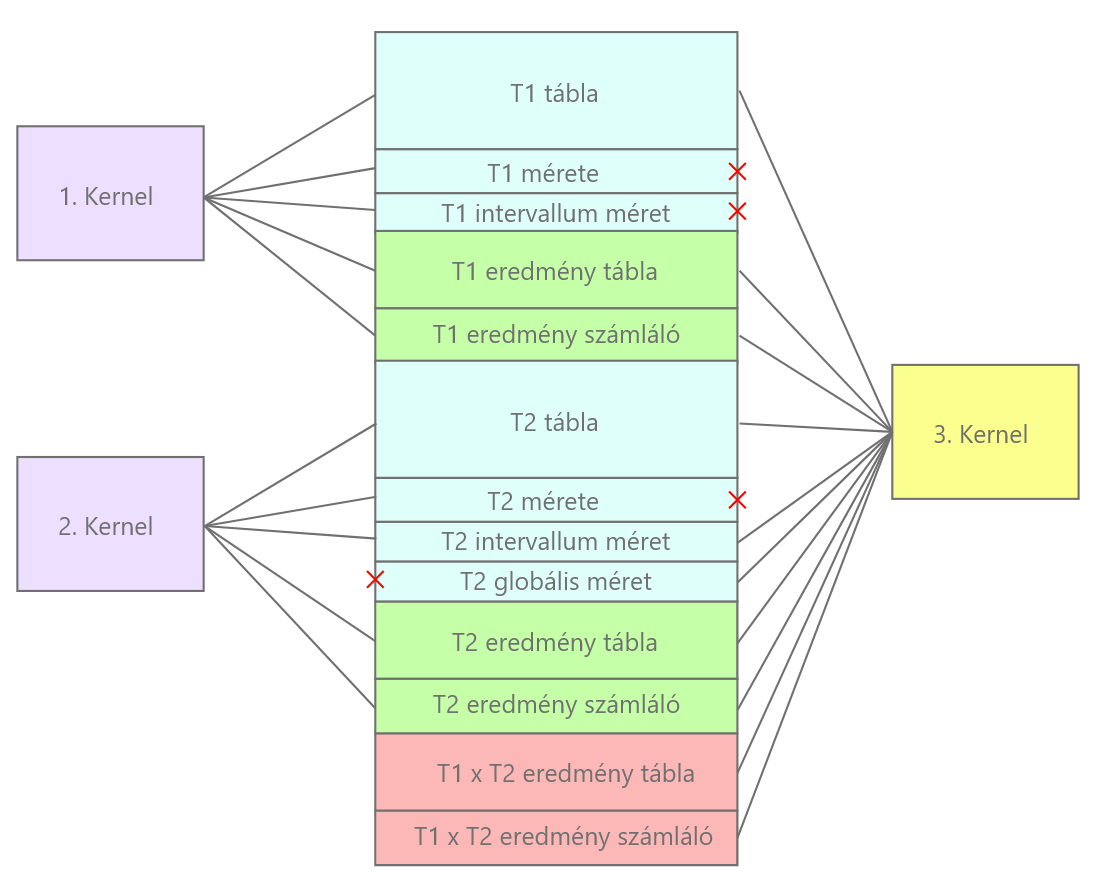
\includegraphics[width=12cm]{images/join_kernels.png}
\caption{Kernelek munkaterületei }
\label{fig:join_kernels}
\end{figure}

Az 1. és 2. kernel az előzőekben taglalt módon előállítja saját eredményeit (zöld rész). 
A 3. kernel megkapja a két táblát, a 2. tábla méretét és az előző két kernel által előállított eredményeket.
Az első eredmény kiolvasási módszer alkalmazásával és a kulcsok figyelésével a két táblát összekapcsoljuk majd előállítjuk az eredményt.
A táblák méretére nincsen szükség, ugyanis az eredmény biztosan nem tartalmaz olyan indexet, ami kívül esne az eredeti táblákon. A második táblánál viszont szükség van a globális méretre is a kiolvasáshoz (\ref{fig:join_kernels}. ábra).
